\documentclass[10pt,a4paper]{article}
\usepackage[margin=2cm]{geometry}
\usepackage{amsmath,amssymb,graphicx,caption,float,hyperref,xcolor}
\hypersetup{colorlinks=true,linkcolor=blue!50!black,urlcolor=blue!50!black}
\captionsetup{font=small,labelfont=bf}
\graphicspath{{../../figures/}}
\title{\vspace{-1.2cm}\textbf{Why reading more helps or protects: the mechanism}\\[2pt]
\large Simulation 2, \texttt{task003-symmetric} and \texttt{task003-nosolution}}
\author{Step 2 of the key-phenomena study (Campaign A); 20 October 2026}
\date{}
\begin{document}
\maketitle
\vspace{-1cm}

\paragraph{Run.} \texttt{results/simulation\_2/2026-10-20\_sim2\_reading\_mechanism}: both setups, 8 memories $\rho$,
$q \in \{3, 6, 9, 12\}$, false controller (target A2) and silent arm, $q_c = 12$, $\lambda_c = 1$, gate on, $B = 30$,
$W = 48$, 1{,}000 paired episodes, each agent's memory recorded every 0.25 and every board post (128 settings,
5.7 GB). The 96 settings at $q = 3, 6, 12$ reproduce the earlier runs exactly. $G$, $D$: as in step 1; all at
$t = 30$. Bars: 95\% intervals.

\begin{figure}[H]
\centering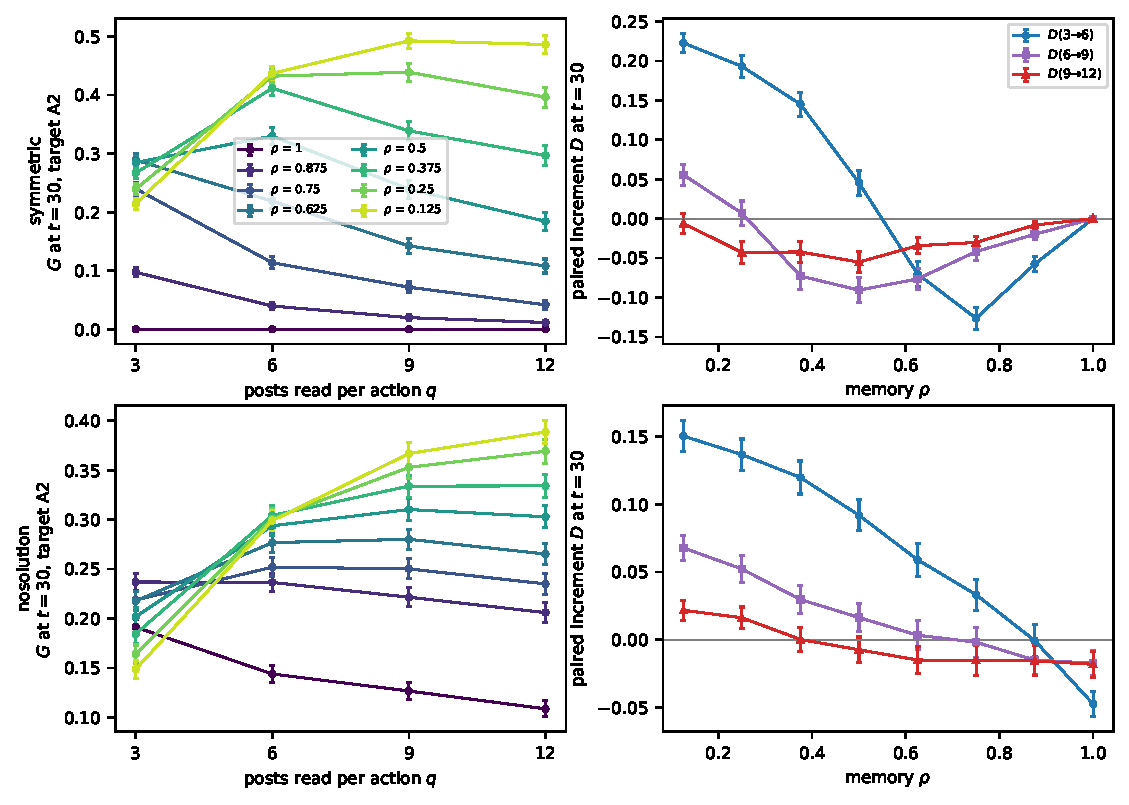
\includegraphics[width=0.95\linewidth]{step2_fig1_G_and_D.pdf}
\caption{Left: $G$ against $q$, one line per $\rho$. Right: $D(3\!\to\!6)$, $D(6\!\to\!9)$, $D(9\!\to\!12)$ against
$\rho$. Top: symmetric; bottom: nosolution.}
\end{figure}

\begin{itemize}\itemsep1pt
\item The controller's best $q$ falls as memory grows: symmetric 9 ($\rho \le 0.25$), 6 ($0.375$--$0.5$), 3
  ($\rho \ge 0.625$); nosolution 12 ($\rho \le 0.375$), 9 ($0.5$--$0.625$), 6 ($0.75$), 3 ($\rho \ge 0.875$).
\item Each further step of $q$ changes $G$ less when agents forget, and turns negative at lower $\rho$.
\end{itemize}

\begin{figure}[H]
\centering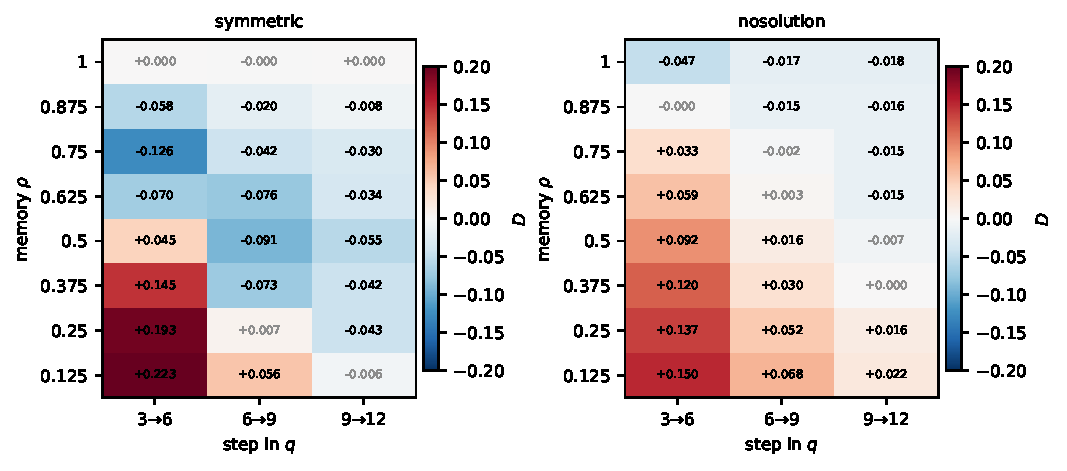
\includegraphics[width=0.85\linewidth]{step2_fig2_D_map.pdf}
\caption{$D$ for each step of $q$ and each $\rho$ (grey number: the 95\% interval includes 0).}
\end{figure}

\begin{itemize}\itemsep1pt
\item Symmetric: $D$ changes sign between $\rho = 0.5$ and $0.625$ ($3\!\to\!6$), $0.25$ and $0.375$ ($6\!\to\!9$),
  $0.125$ and $0.25$ ($9\!\to\!12$).
\item Nosolution: between $0.75$ and $0.875$ ($3\!\to\!6$), around $0.625$--$0.75$ ($6\!\to\!9$), around
  $0.375$--$0.5$ ($9\!\to\!12$).
\item The crossover contour descends smoothly, by 0.125--0.25 in $\rho$ per step of $q$, and lies about 0.3 higher in
  $\rho$ without a proof. With the equidistant $q$ grid it is a gradual slope, not a sharp edge.
\end{itemize}

\begin{figure}[H]
\centering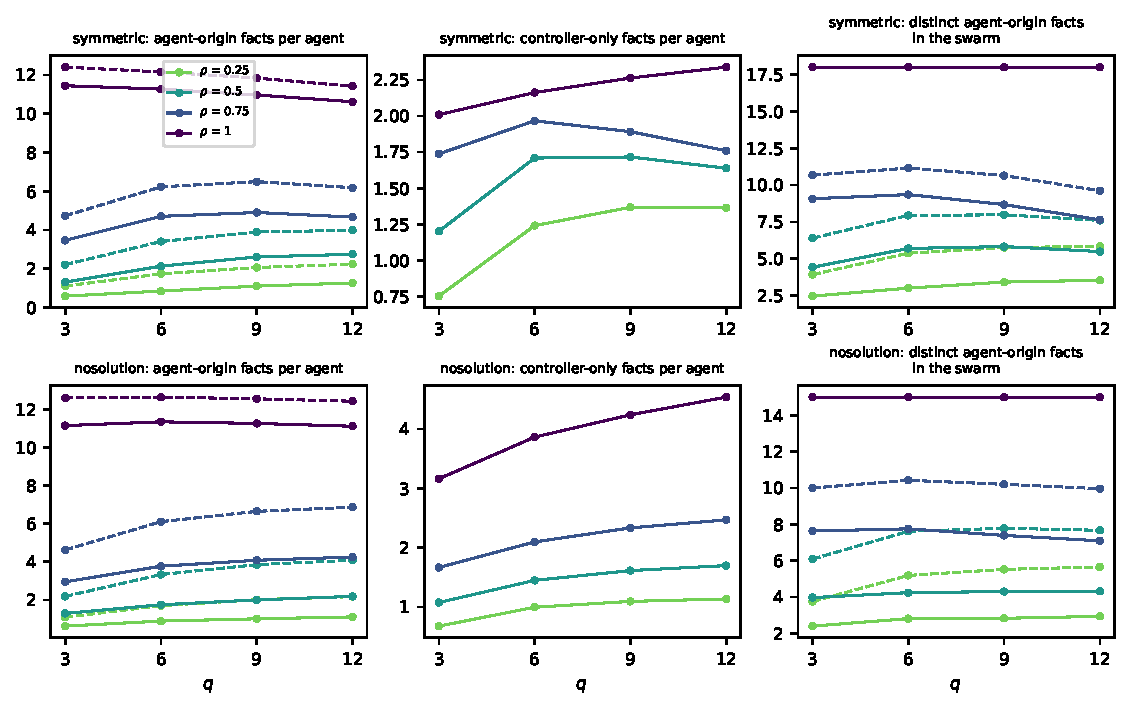
\includegraphics[width=0.95\linewidth]{step2_fig3_memory.pdf}
\caption{At $t = 30$, against $q$: agent-origin facts per agent, controller-only facts per agent, and distinct
agent-origin facts held by anyone; false arm solid, silent dashed; $\rho = 0.25, 0.5, 0.75, 1$.}
\end{figure}

\begin{itemize}\itemsep1pt
\item Reading more lets agents hold more of their own evidence in both arms (false arm, $q = 3 \to 12$: up to
  $\times 2.2$ in symmetric and $\times 1.8$ in nosolution).
\item At low $\rho$ it also brings in more of the controller's facts (symmetric $\rho = 0.25$: 0.75 $\to$ 1.36 per
  agent); in symmetric at high $\rho$ these level off or fall ($\rho = 0.75$: 1.74, 1.97, 1.89, 1.76).
\item The controller lowers the swarm's coverage of agent-origin facts at every $q$ and $\rho < 1$, by 0.9--2.4
  (symmetric) and 1.1--3.5 (nosolution) distinct facts.
\item Counts alone do not decide the sign: in nosolution at $\rho = 1$ agents hold more controller-only facts as $q$
  grows (3.2 $\to$ 4.5) while $G$ falls.
\end{itemize}

\begin{figure}[H]
\centering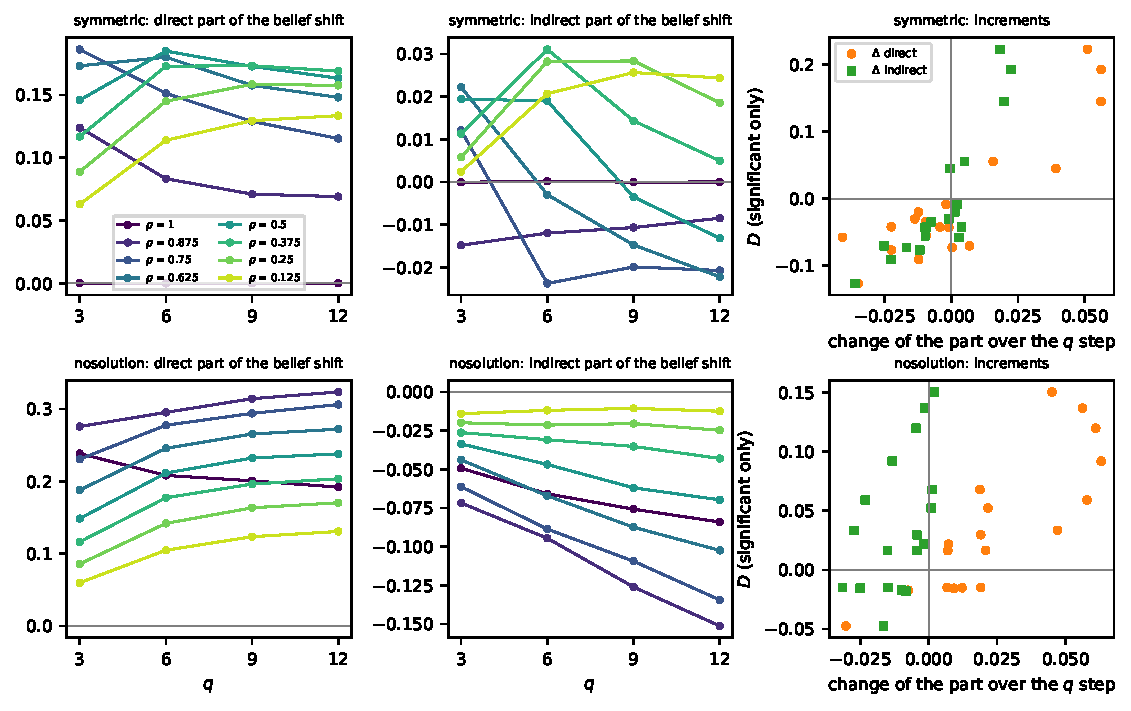
\includegraphics[width=0.95\linewidth]{step2_fig4_split.pdf}
\caption{The false arm's extra belief in A2 over the silent arm, split exactly into a \emph{direct} part (what the
controller-only facts add: belief from all remembered facts minus belief from the agent-origin facts alone) and an
\emph{indirect} part (which agent-origin facts are kept: belief from them minus the silent arm's belief), against
$q$, one line per $\rho$. Right: the change of each part over a $q$ step against $D$ (significant $D$ only).}
\end{figure}

\begin{itemize}\itemsep1pt
\item The sign of $D$ follows the change of the direct part in 17 of 19 significant increments (symmetric) and 15 of
  19 (nosolution); correlations 0.89 and 0.83.
\item Nosolution: reading more raises the direct part at every $\rho < 1$ (spreading), while the indirect part falls,
  most at high $\rho$ ($-0.015$ to $-0.031$ per step at $\rho \ge 0.625$; integration of the agents' own evidence).
  $D$ turns negative where the indirect fall outweighs the direct rise.
\item Symmetric: at $\rho \ge 0.75$ the direct part falls with $q$ at every step ($-0.002$ to $-0.041$): held alongside
  more agent facts, the controller's facts move beliefs less (dilution). At $\rho \le 0.375$ both parts rise from $q = 3$ to 6.
\item The two-function hypothesis is supported: reading spreads the controller's selection and integrates the agents'
  evidence; memory sets which wins.
\end{itemize}

\paragraph{Caveat.} The split is on mean beliefs; $G$ is on votes (drawn from beliefs). They agree in sign. One world
per setup, $N = 24$.

\end{document}
